\documentclass{article}
% packages
\usepackage[margin=1 in]{geometry}
\usepackage{indentfirst}
\usepackage{titlesec}
\usepackage{enumitem}
\usepackage{adjustbox}

% natbib package
\usepackage[square,sort,comma]{natbib}
\usepackage[hyphens,spaces,obeyspaces]{url}
\setcitestyle{citesep={;}}

%math package
\usepackage{amsmath}
\usepackage{mathtools}

% Use Links
\usepackage{xcolor}
\usepackage[colorlinks=true ,citecolor=blue, urlcolor=blue,urlbordercolor={1 0 0}]{hyperref} 

% Set the spacing between paragraphs and have a small paragraph indentation
\setlength\parskip{1em}
\setlength\parindent{2em}
\titlespacing{\section}{0pt}{\parskip}{-\parskip}
\titlespacing{\subsection}{0pt}{\parskip}{-\parskip}
\titlespacing{\subsubsection}{0pt}{\parskip}{-\parskip}

% graphics path
\usepackage{graphicx}
\graphicspath{{graphics/}}

\title{HUDM 5126 Linear Models and Regression Analysis Final Project\footnote{This document is written in \LaTeX. Please do not cite or circulate this preliminary draft.}\\
Modeling and Prediction for Movies}
\author{Yifei Dong\footnote{Department of Human Development, Teachers College, Columbia University: \href{mailto: yd2564@tc.columbia.edu}{yd2564@tc.columbia.edu}}}
\date{Dec 21 2020}

\begin{document}
\maketitle

\section{Data and Research Question}
\smallskip
The data set used in this project 'movies' is taken from Duke University Department of Statistical Science. There data were originally obtained from IMDB and Rotten Tomatoes. This data set is comprised of 32 variables and 651 randomly sampled movies produced and released before 2016. It is worth to notice that this is an observational study and researcher are trying to capture most of significant factors of a movie, such as its genre (Action \& Adventure, Comedy, Documentary, Drama, Horror etc), runtime, whether or not the movie was nominated for a best picture Oscar, critic score and audience score on Rotten Tomatoes, and whether or not the movie is in the Top 200 Box Office list on BoxOfficeMojo. Nevertheless, due to the fact that the data does not result from an experiment study, we cannot establish causality with any results from the data. 

In terms of generalizability, based on the box plot of the number of movies released in theater
per year (Figure~\ref{fig: 1}), 75\% of the years in  the data set have less than 20 movies
released. Based on the rule of thumb, we need at least 30 observations to generalize our results 
to the whole population. Therefore, we could not generalize our research results to all U.S movies 
produced and released in each year. However, due to the fact that this data set consists of 651 
randomly sampled movies, and the total number of observations (n=651) in this data set is well 
below 10\% of all movies produced and released in the United Sates before 2016, we could 
safely generalize this data to the population of interest. 

\begin{figure}[htbp]
\begin{center}
\caption{Distribution of the number of movies released in theater per year}
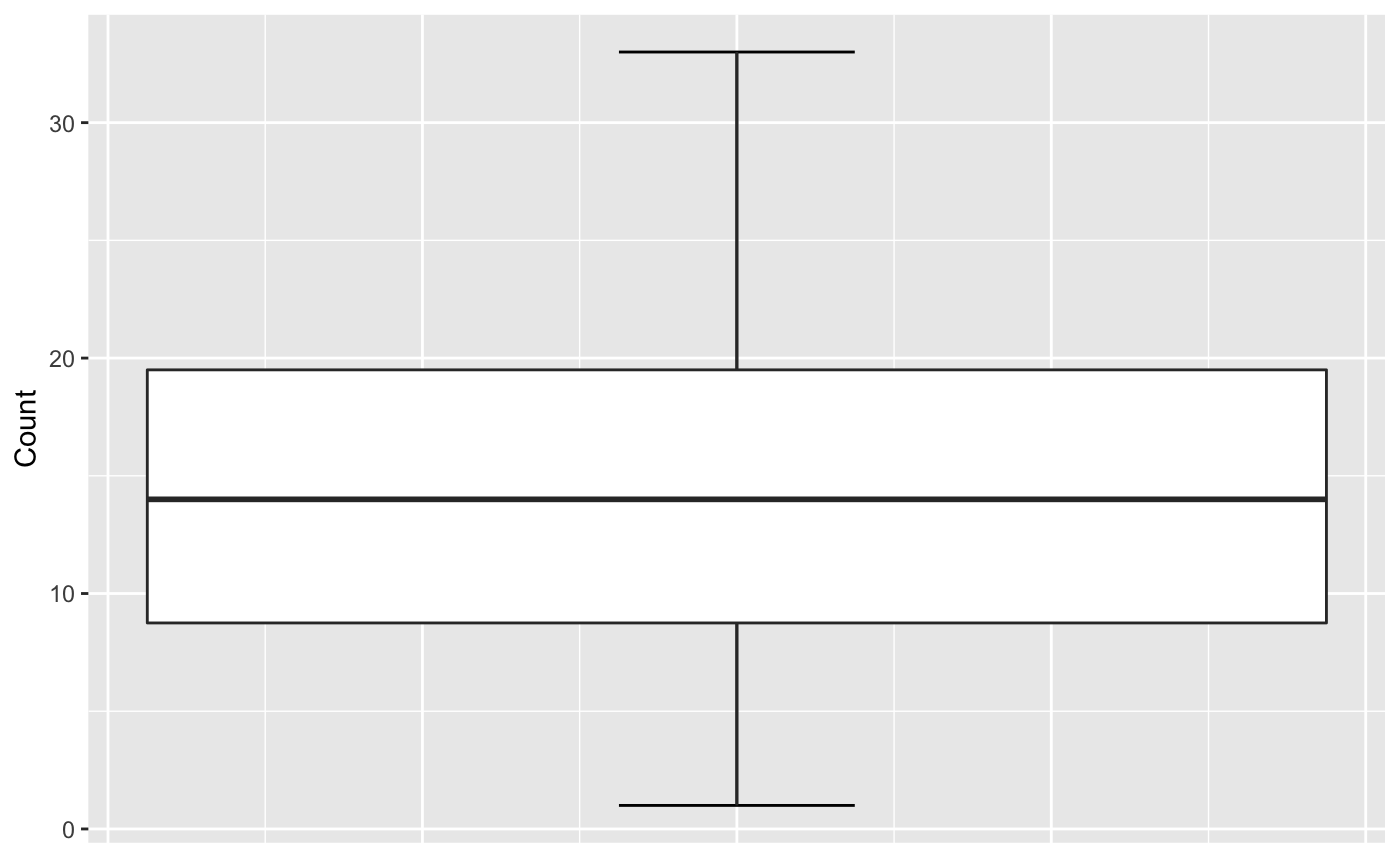
\includegraphics[scale=0.3]{data_a.png}
\label{fig: 1}
\end{center}
\end{figure}

In addition, according to the codebook for this data set \citep{Runde2020}, some of these variables are only there for informational purposes and do not make any sense to include in a statistical analysis, such as the director and first main actor/actress's name in the movie.  On this occasion, those kinds of variables could be omitted from my analysis.

The main research question in this project is that what are the driving factors for determining the popularity of a movie, as measured by the audience score on Rotten Tomatoes. The following variables will be removed from our analysis due to their informational purposes, which are:

\vspace{-0.5cm}
\begin{itemize}
\setlength\itemsep{-0.5em}
\item title: Title of movie
\item studio: Studio that produced the movie
\item director: Director of the movie
\item actor1: First main actor/actress in the abridged cast of the movie
\item actor2: Second main actor/actress in the abridged cast of the movie
\item actor3: Third main actor/actress in the abridged cast of the movie
\item actor4: Fourth main actor/actress in the abridged cast of the movie
\item actor5: Fifth main actor/actress in the abridged cast of the movie
\item imdb\_url:  Link to IMDB page for the movie
\item rt\_url: Link to Rotten Tomatoes page for the movie
\end{itemize}

Also, the time-relevant variables are also exclude from our analysis, such as specific years, month, and day the movie is released in theaters and on DVD. After removing those variables, I select the following variables to start the analysis:

\vspace{-0.5cm}
\begin{itemize}
\setlength\itemsep{-0.5em}
\item title\_type: Type of movie (Documentary, Feature Film, TV Movie)
\item genre: Genre of movie (Action \& Adventure, Comedy, Documentary, Drama, Horror, Mystery \& Suspense, Other)
\item runtime: Runtime of movie (in minutes)
\item mpaa\_rating: MPAA rating of the movie (G, PG, PG-13, R, Unrated)
\item imdb\_rating: Rating on IMDB
\item imdb\_number\_votes: Number of votes on IMDB
\item critics\_rating: Categorical variable for critics rating on Rotten Tomatoes (Certified Fresh, Fresh, Rotten)
\item critics\_score: Critics score on Rotten Tomatoes
\item audience\_rating: Categorical variable for audience rating on Rotten Tomatoes (Spilled, Upright)\footnote{This actually refers to the Popcorn bucket icon on Rotten Tomatoes. Specifically, when at least 60\% of users give a movie or TV show a star rating of 3.5 or higher, a full popcorn bucket is displayed to indicate its Fresh status (Upright). When less than 60\% of users give a movie or TV show a star rating of 3.5 or higher, a tipped over popcorn bucket is displayed to indicate its Rotten Status (Spilled). See \url{https://www.rottentomatoes.com/about}}
\item best\_pic\_nom: Whether or not the movie was nominated for a best picture Oscar (no, yes)
\item best\_pic\_win: Whether or not the movie won a best picture Oscar (no, yes)
\item best\_actor\_win: Whether or not one of the main actors in the movie ever won an Oscar (no, yes) – note that this is not necessarily whether the actor won an Oscar for their role in the given movie
\item best\_actress\_win: Whether or not one of the main actresses in the movie ever won an Oscar (no, yes) – not that this is not necessarily whether the actresses won an Oscar for their role in the given movie
\item best\_dir\_win: Whether or not the director of the movie ever won an Oscar (no, yes) – not that this is not necessarily whether the director won an Oscar for the given movie
\item top200\_box: Whether or not the movie is in the Top 200 Box Office list on BoxOfficeMojo (no, yes)
\end{itemize}

After checking in R, the data set has one observations with missing value for the 
variable "runtime", which is the movie titled as "The End of America". Therefore, I 
decide to remove this data from our data set. Therefore, the final data set used in 
this project has 650 observations in total.

\newpage
\section{Exploratory Data Analysis}
Before modeling, it is necessary to conduct some exploratory data analysis so that we could get some general idea of movies' characteristics in our data set. It is quite clear that the majority of the predictor variables are categorical variables, therefore, barplot could be chosen as a useful data visualization tool to summarize the distribution of those categorical variables. In terms of numerical variables, histograms or boxplots are better visualization techniques.

\subsection{Categorical Variables}
I create barplots for each categorical variables in the data set. According to Figure~\ref{fig: 2}, among 650 movies, 591 are feature films, and 307 (47.23\%) of those movies are rated by critics on Rotten Tomatoes as "Rotten", which means they are not favorable by professional movie critics. On the contrary, 375 out of 650 movies are rated as "Upright" by audience, indicating those movies are favorable by audiences. Therefore, I do observe some differences on ratings between professional critics and audiences. Moreover, in terms of genre of movies, based on Figure~\ref{fig: 3}, 305 out of 650 (46.92\%) are drama. 

\begin{figure}[htbp]
\begin{center}
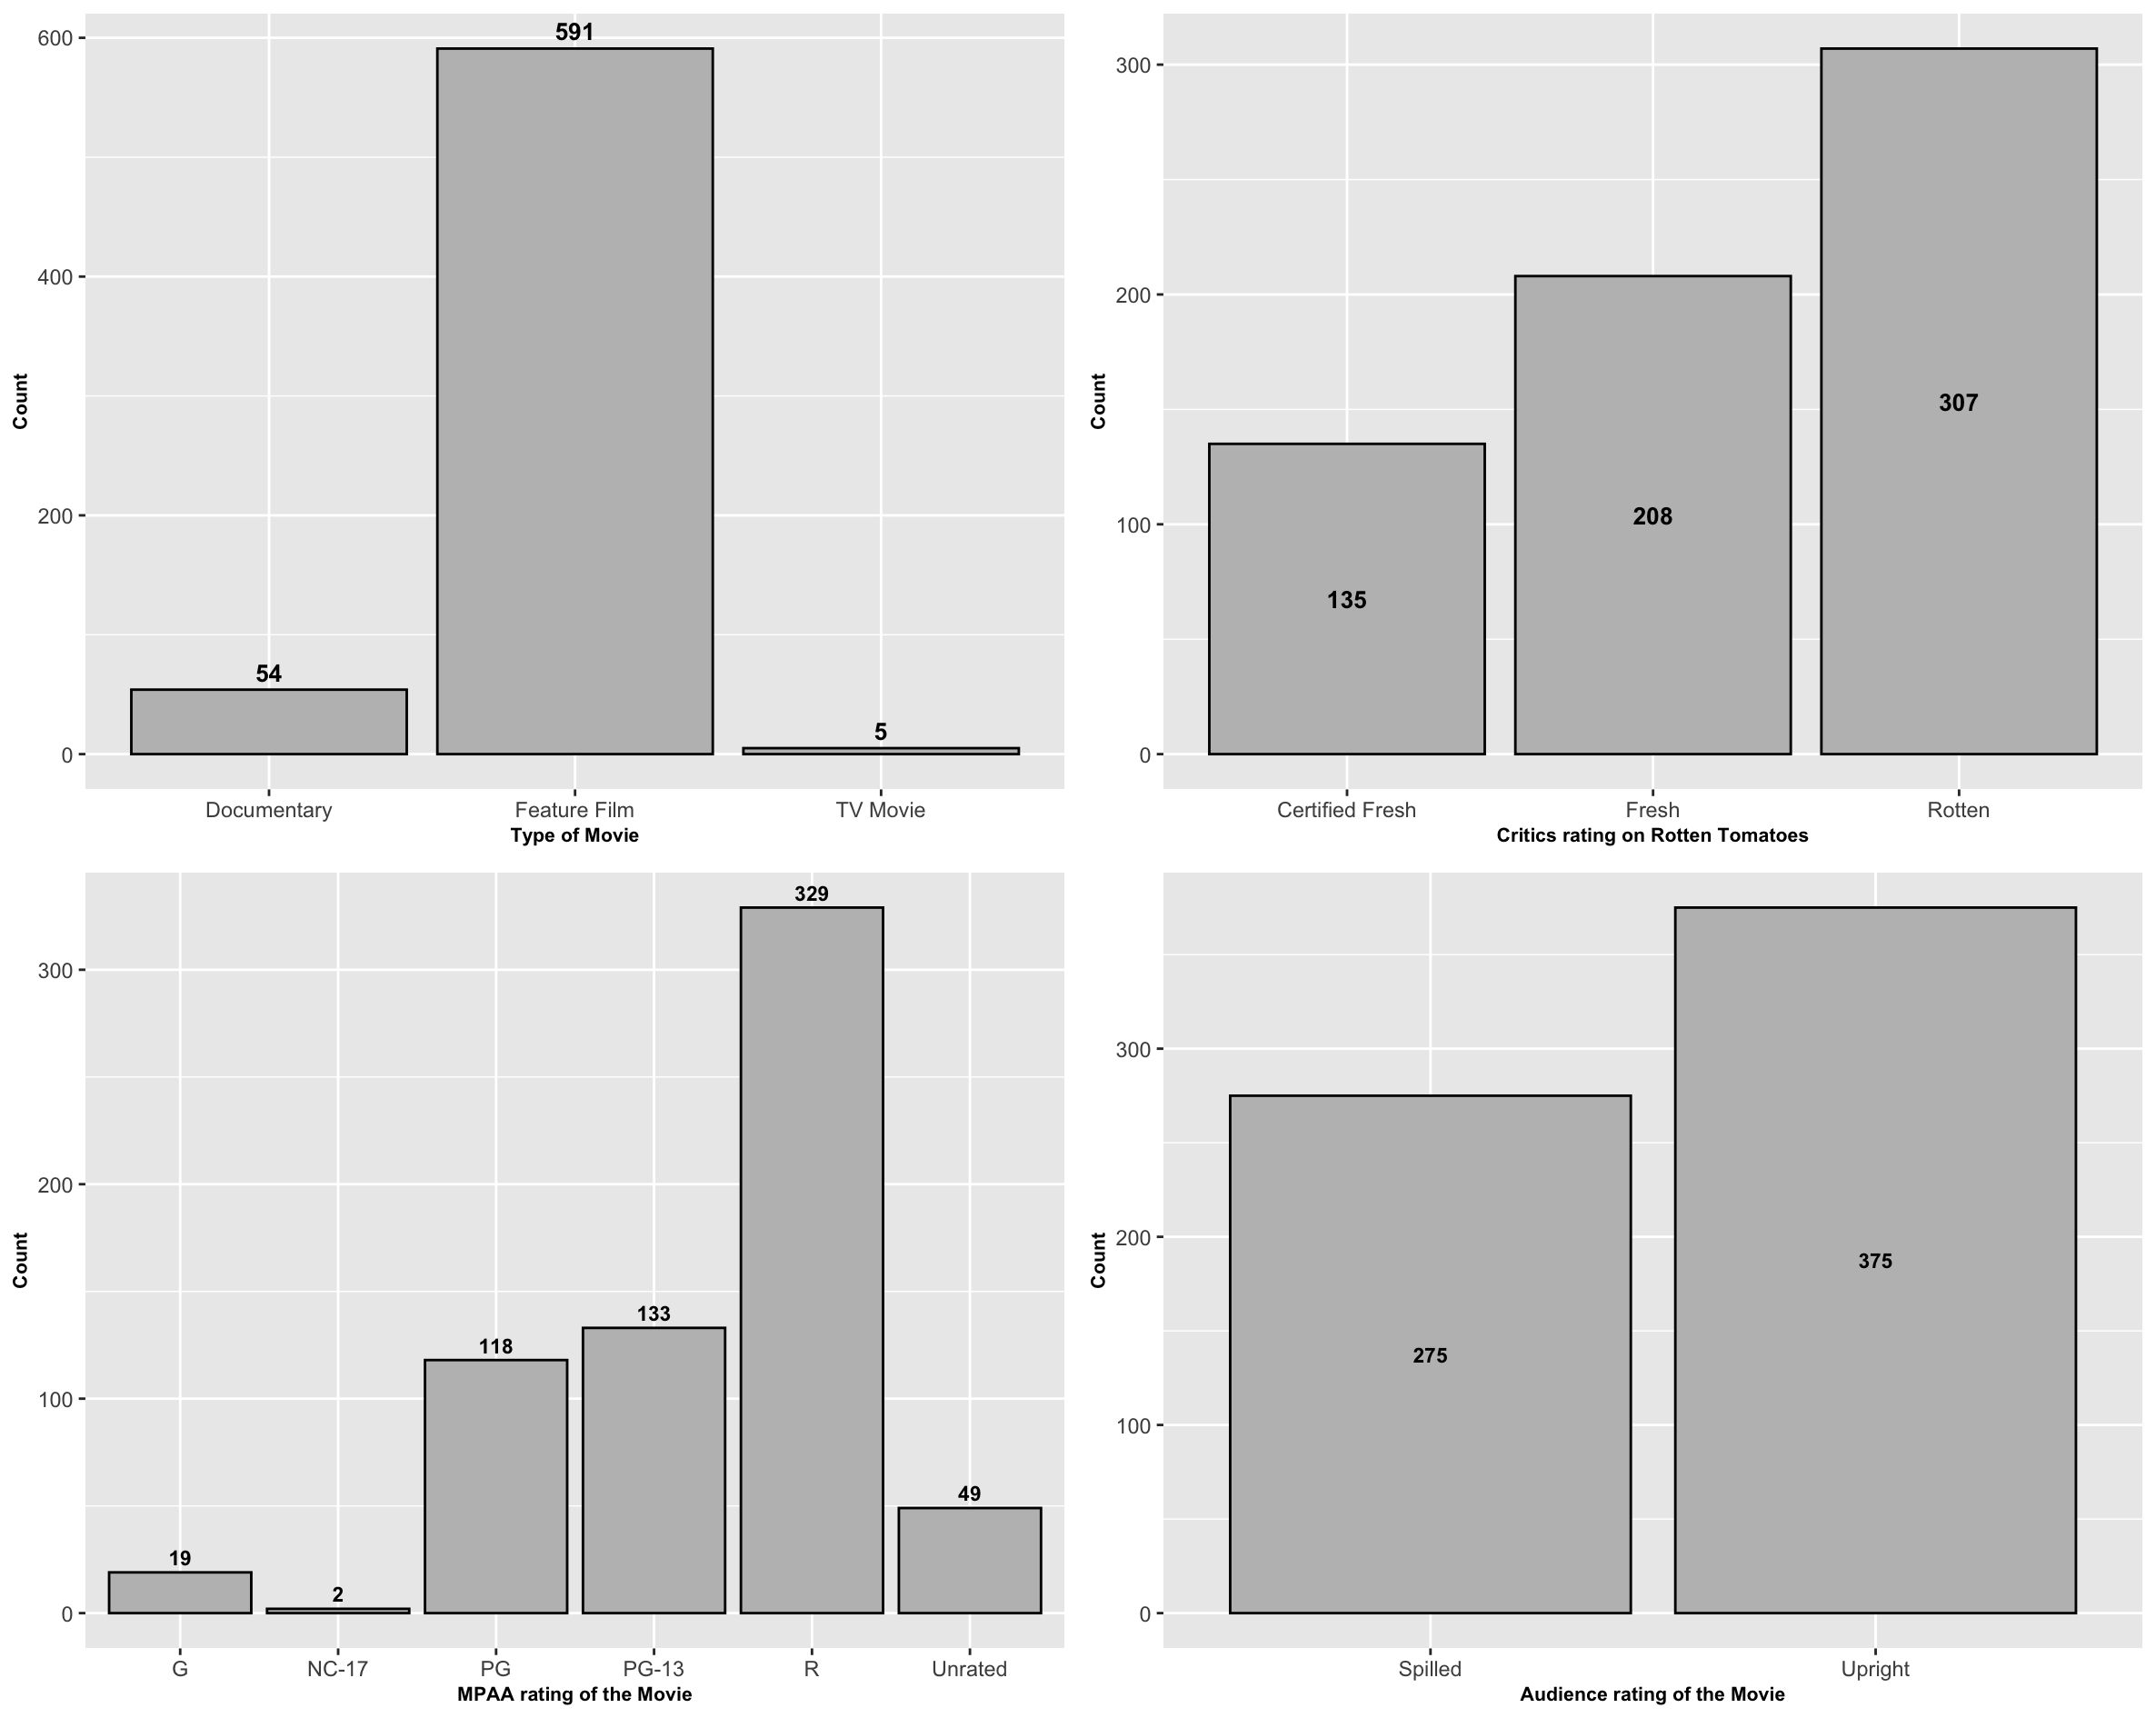
\includegraphics[scale=0.20]{eda_1.png}
\caption{Barplots for Categorical Variables: Type of Movie, Critics rating on Rotten Tomatoes, MPAA rating of the Movie, and Audiences Rating on Rotten Tomatoes}
\label{fig: 2}
\end{center}
\end{figure}

\newpage

\begin{figure}[htbp]
\begin{center}
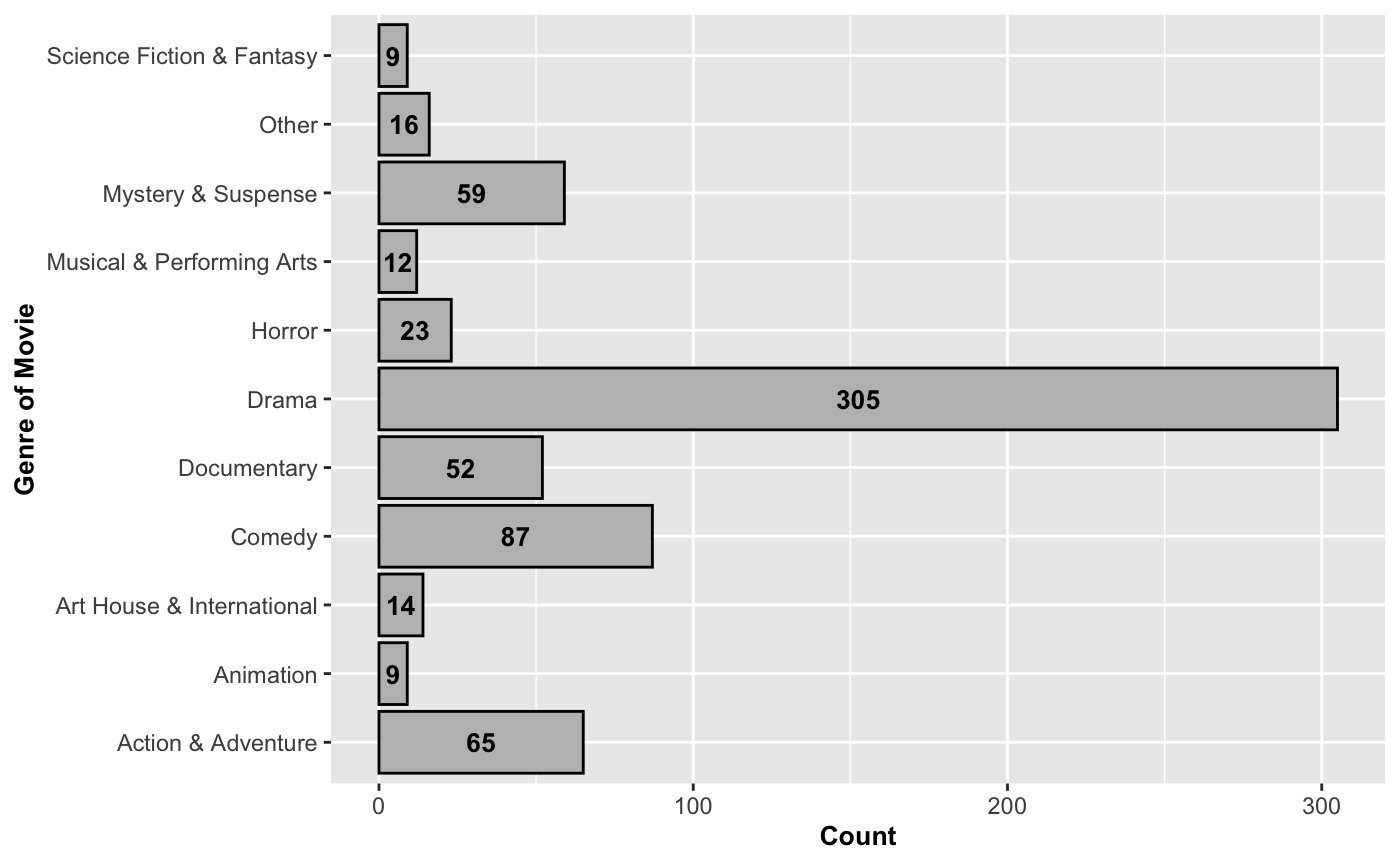
\includegraphics[scale=0.3]{barplot_genre.png}
\caption{Barplot for Genre of Movies }
\label{fig: 3}
\end{center}
\end{figure}

Figure~\ref{fig: 4} lists another six barplots for the categorical variables. Based on those plots, it is clear that the majority of movies in the data set seems neither won an Oscar Best Pictures nor were nominated for the same award. In addition, the data set also consists of movies with the main actors/actresses and directors not having won an Oscar so far. Finally, nearly 97.67\% of the movies are not  in the Top 200 Box Office list on BoxOfficeMojo. 

\begin{figure}[htbp]
\begin{center}
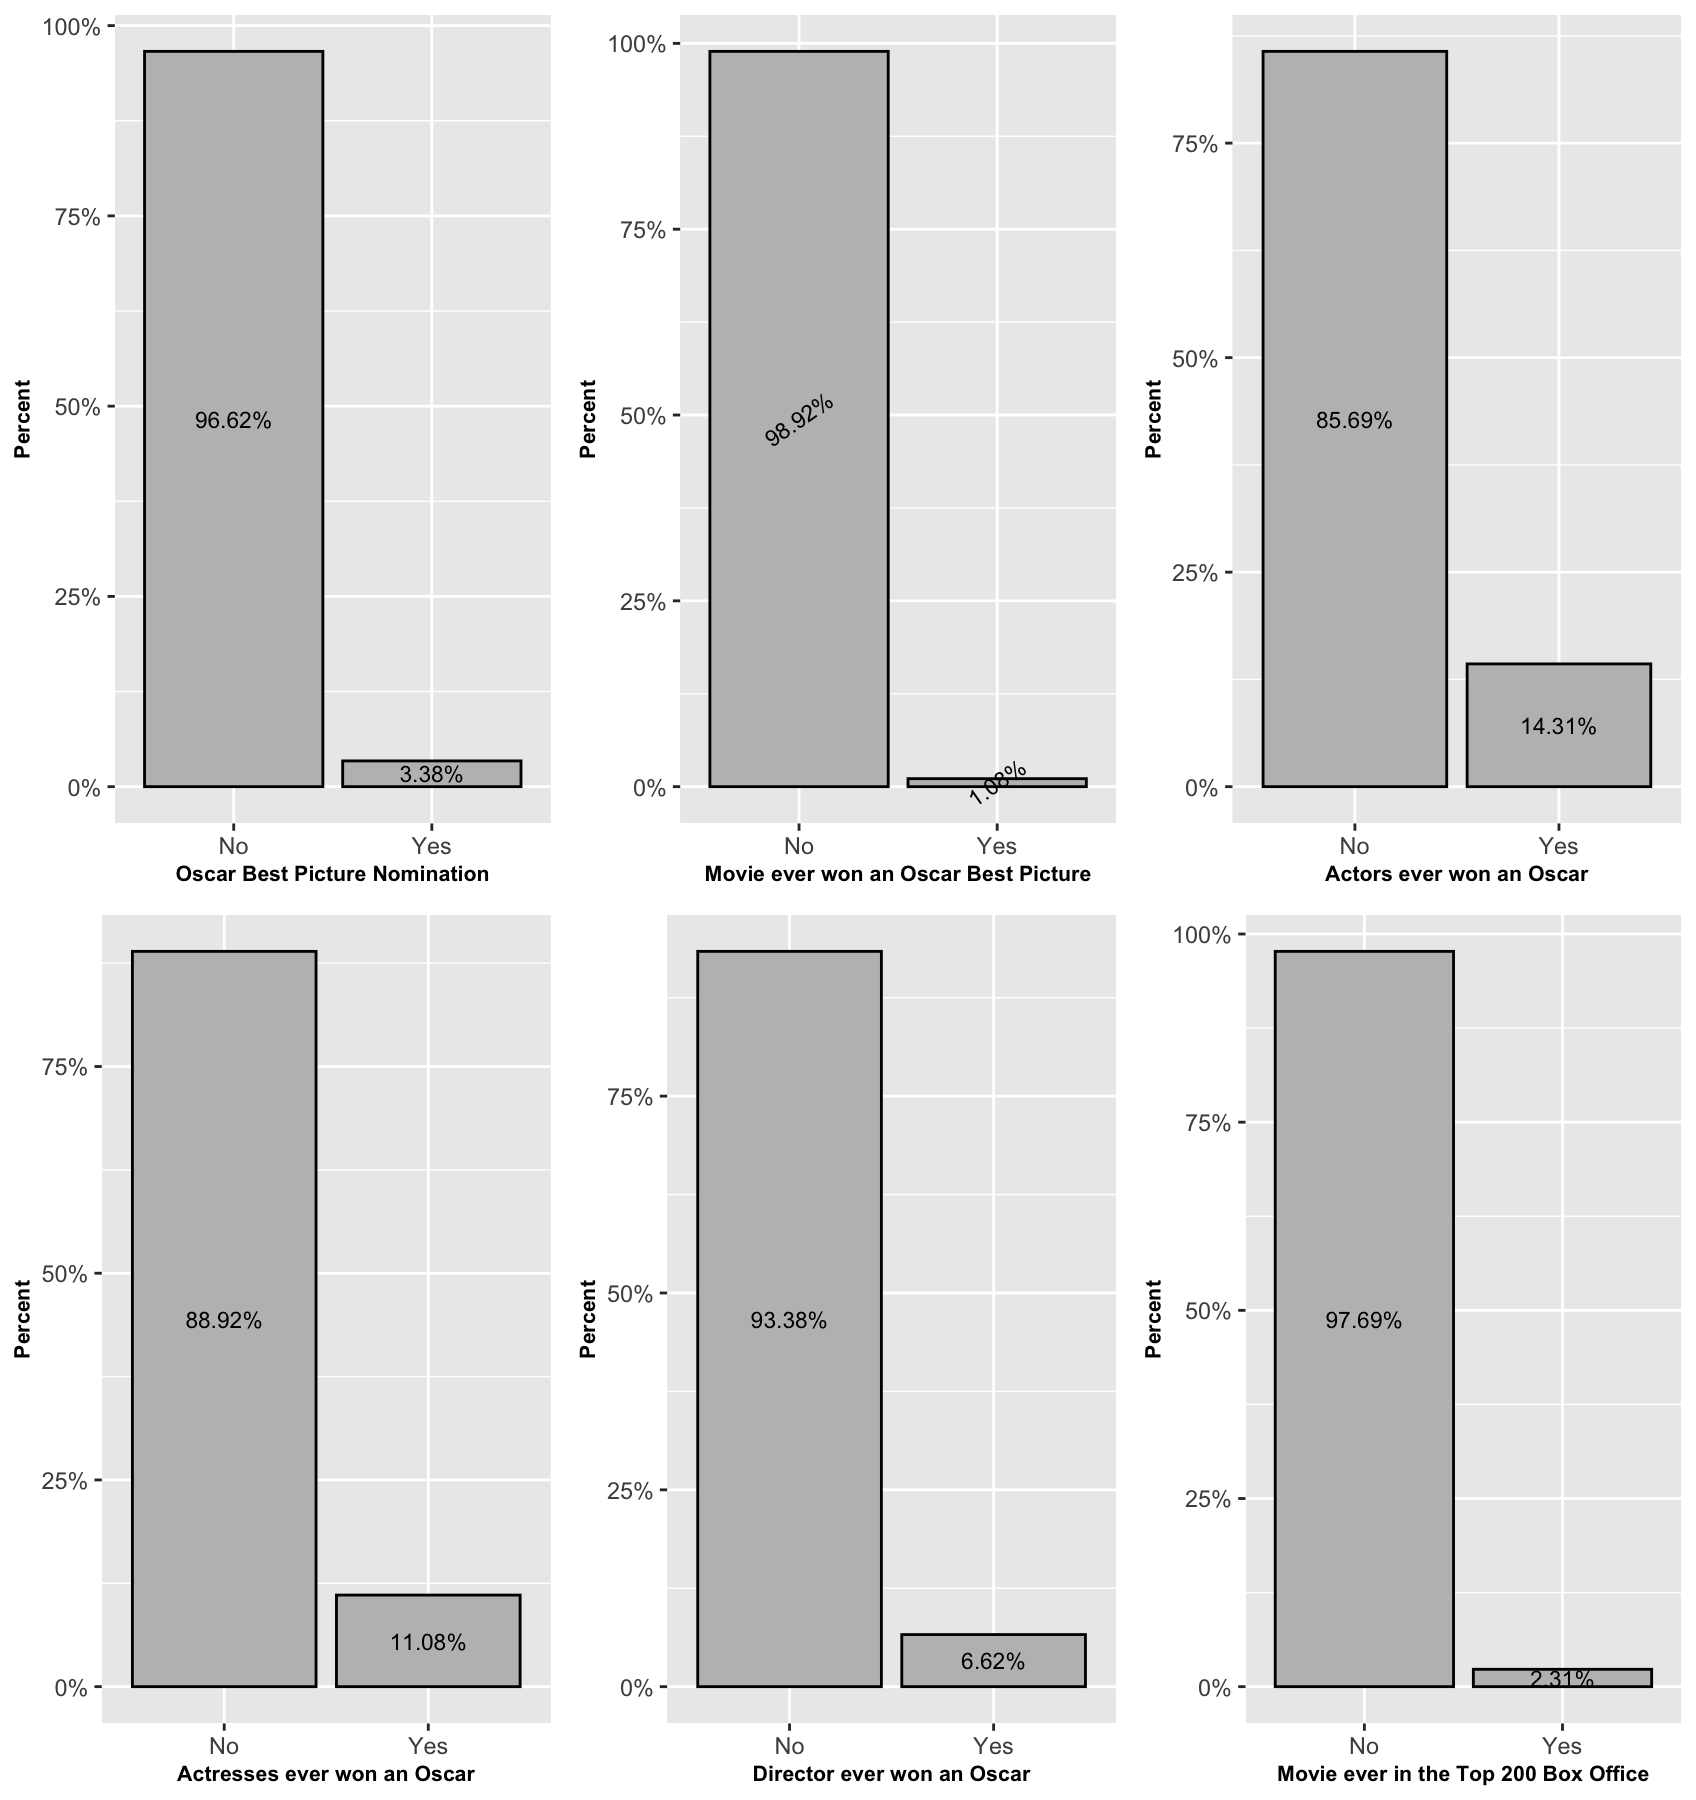
\includegraphics[scale=0.25]{eda_2.png}
\caption{Barplots for Categorical Variables (Continued): Oscar Best Picture Nomination, Oscar Best Picture Won Status, Whether or not One of the Main Actors/Actresses in the Movie ever Won an Oscar, Oscar Director Award Won Status, and Whether or not the Movie is in the Top 200 Box Office}
\label{fig: 4}
\end{center}
\end{figure}

\subsection{Numerical Variables}
\smallskip
\subsubsection{Response Variable: Audience Score}
Figure~\ref{fig: 5} is the histogram of the response variable in this project, the audience 
score of the movie on Rotten Tomatoes. The median of the response variable, audience
score is 65. 25\% of the movies in the data set have audience score higher than 80 and 
25\% of the movies have audience score lower than 46. The lowest audience score in the 
data set is 11 and the highest is 97. Also, due to the fact that mean of audience score is 
less than the median of audience score, we have a left-skewed distribution.

\subsubsection{Other Numerical Variables}
Figure~\ref{fig: 6} lists histograms for other four numerical variables, which are movie's run time, IMDB rating, number of votes, and critics scores on Rotten Tomatoes. The run time, IMDB number of votes have a right-skewed distribution, while IMDB rating and critics scores on Rotten Tomatoes have left-skewed distributions. It may be reasonable to do some data transformations in regard to those skewed distributed variables. But I will leave those variables until I perform model selection and diagnostics.

\begin{figure}[htbp]
\caption{Histogram for Response Variable: Audience Score on Rotten Tomatoes}
\begin{center}
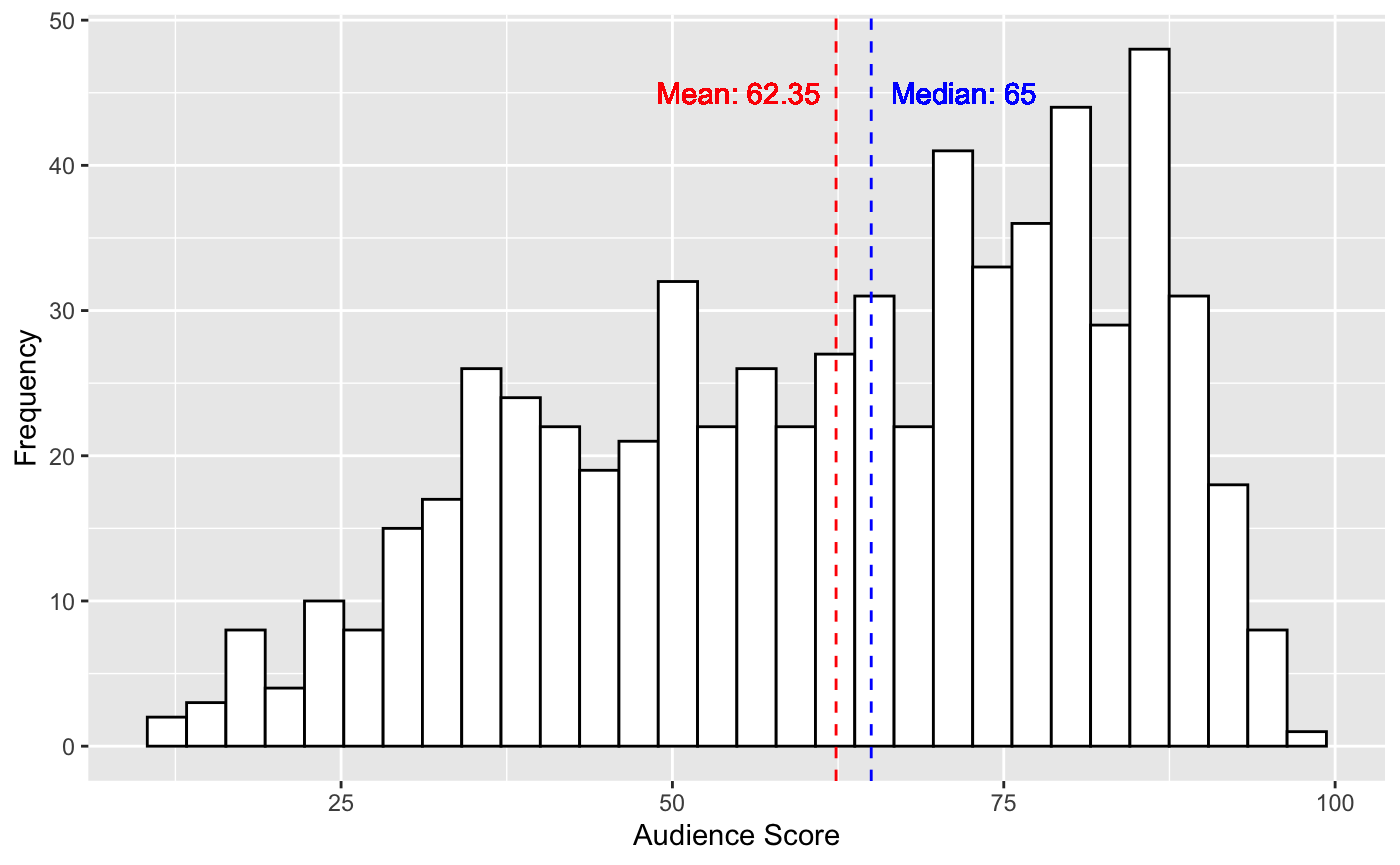
\includegraphics[scale=0.3]{response_variable.png}
\label{fig: 5}
\end{center}
\end{figure}

\begin{figure}[htbp]
\begin{center}
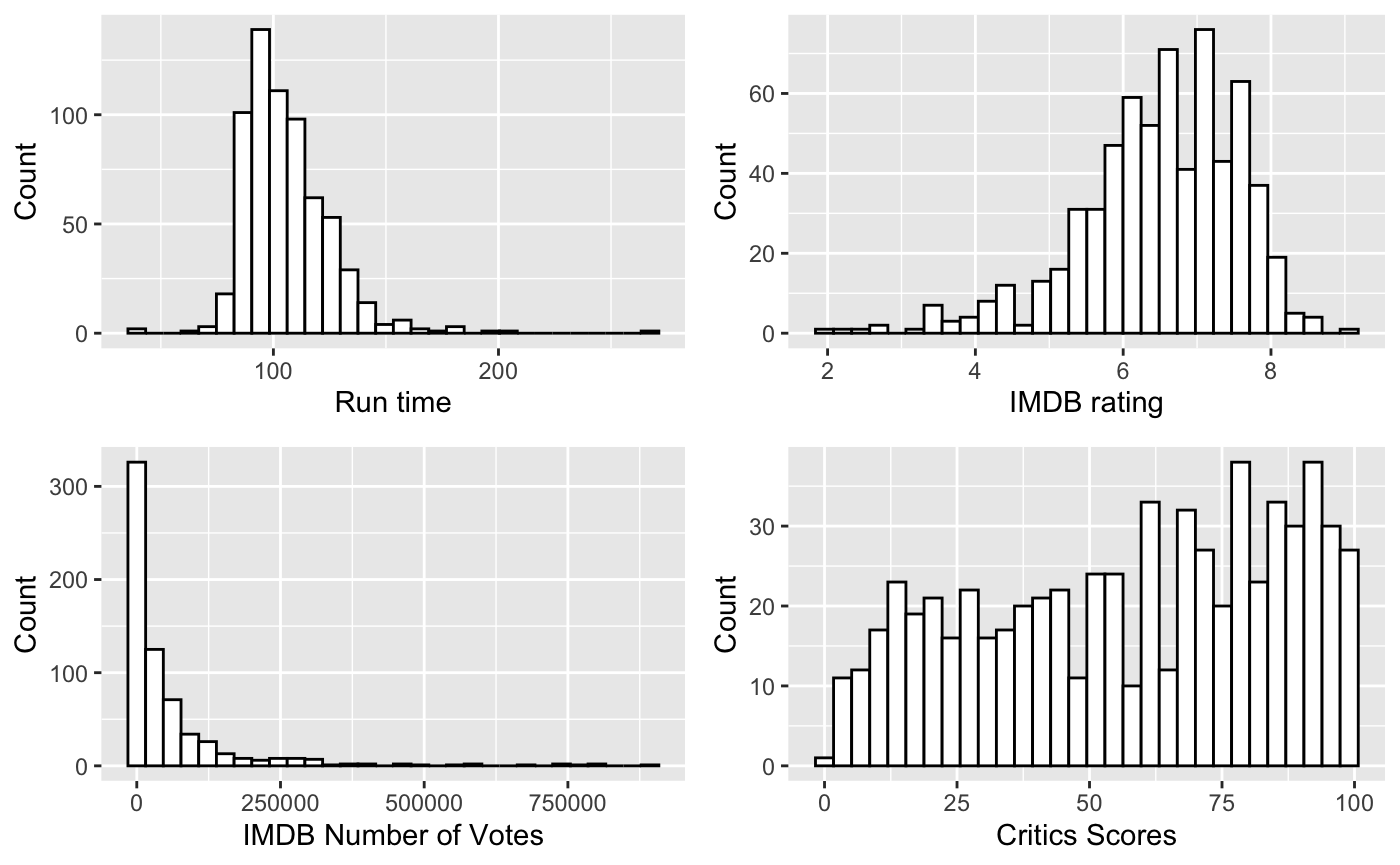
\includegraphics[scale=0.30]{other_numerical.png}
\caption{Histogram of Run time, IMDB rating, IMDB number of Votes, and Critics Scores on Rotten Tomatoes}
\label{fig: 6}
\end{center}
\end{figure}

\newpage
\subsection{Distribution of Response Variable across Various Categorical Variables}
The next step is to get a sense of the distribution of movies data set in terms of the audience score (response variable) as grouped by various levels of the relevant categorical variables. By doing this step in the Exploratory Data Analysis process, we cannot only get a sense of important trends of the data, but also being able to get a sense of the relationship between the response variable and categorical predictor variables. Specifically, we could gauge the sign of slope coefficient for each categorical predictor variable as well as the potential statistical significance of those predictors in predicting the response variable. This step can be done by constructing boxplots for the audience score as grouped by the selected categorical variables.

\begin{figure}[htbp]
\begin{center}
\caption{Boxplots of Audience Score vs. Genre, and Audience Score v.s MPAA Rating}
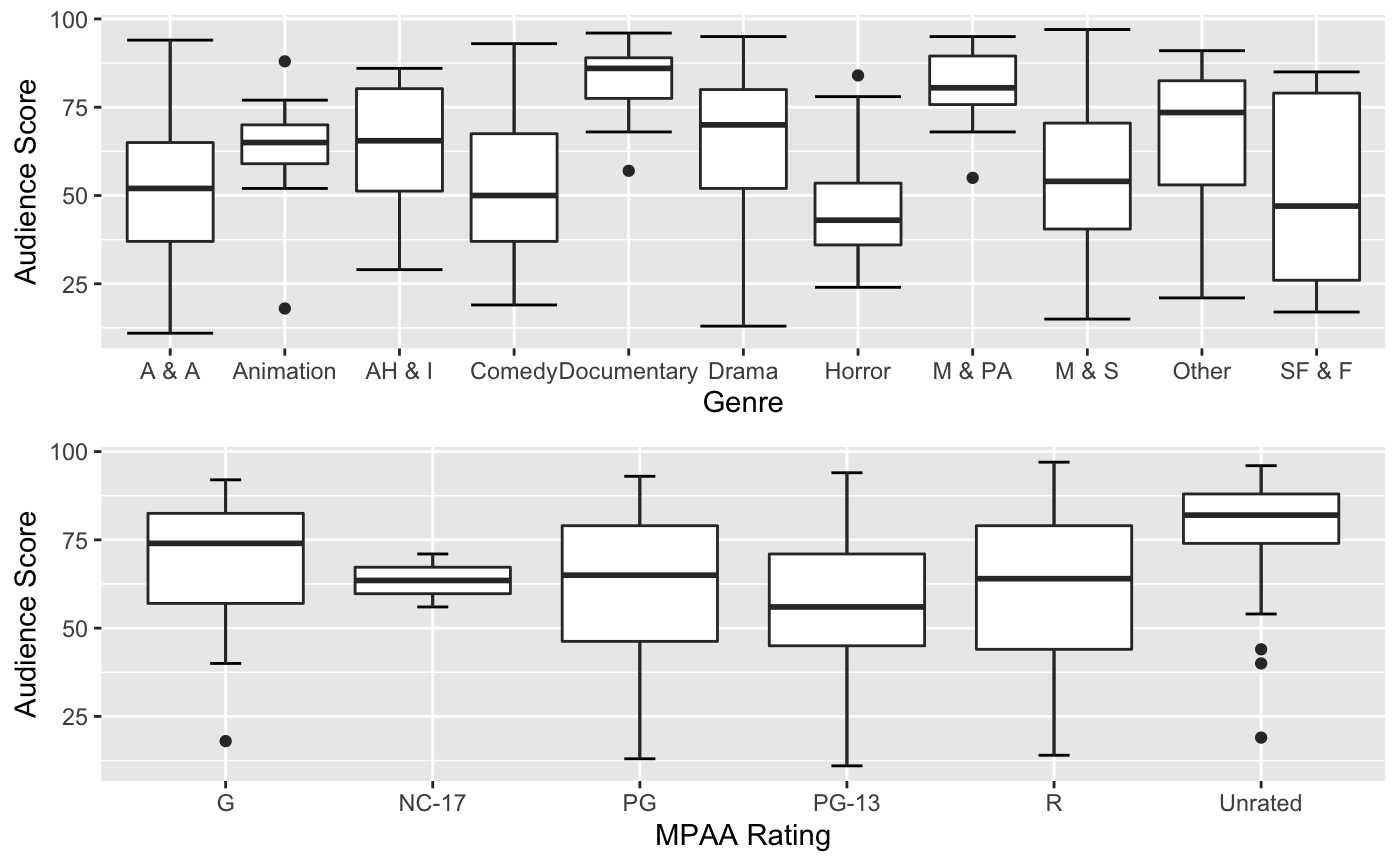
\includegraphics[scale=0.32]{boxplot1.png}
\label{fig: 7}
\end{center}
\end{figure}

According to Figure~\ref{fig: 7}, movies with genres, such as Documentary, Drama, Musical 
and Performing Arts tend to have higher audience scores, while movies with Horror genre are 
less popular. In terms of MPAA Rating, movies that are unrated expect to have higher audience scores, while movies rated as 'PG-13' seem to have lower audience scores.

The boxplot (Figure~\ref{fig: 8} upper left) depicting the distribution of audience score by whether or not the movie received an Oscar Best Picture Nomination conveys the fact that movies that receive a Best Picture Nomination tend to have a higher audience score in comparison to those movies that have not received such nomination. Similarly, the boxplot (Figure~\ref{fig: 8} upper right) depicting the distribution of audience score by whether or not the movie won an Oscar Best Picture Award coveys the similar fact that movies that won a Best Picture Award tend to have a higher audience score in comparison to those movies that have not won a Best Picture Award. For movies not won a Best Picture Award, the distribution of the audience score is fairly symmetric since the median is somewhat located near the center of the box. Nevertheless, the distribution of audience score for movies that won a Best Picture has a right-skewed distribution since the longer part of the box is above the median, indicating that Best Picture Winning movies are likely to receive audience scores higher than the median level. Moreover, there is a potential outlier in this category with audience score  69 but does received a Best Picture Award. 

The boxplot (Figure~\ref{fig: 8} lower left) depicting the distribution of audience score by whether or not the movie is included in the Top 200 Box Office indicates the fact that movies that were included in this list tend to receive a higher audience score compared to movies that were not included in this list. For movies that were not included in the Top 200 Box Office list, the distribution of the audience score is fairly symmetric due to the fact that the median is located near the center of the box. On the contrary, the distribution of audience scores for movies that were included in the list seems skewed to the left as the longer part of the box is below the median. This means that movies feature in the Top 200 Box Office list are likely to receive lower audience scores compared to the median level.

\begin{figure}[htbp]
\begin{center}
\caption{Boxplots of Audience Score vs. Oscar Best Picture Nomination, Audience Score vs. Oscar Best Picture Win, Audience Score vs. Top 200 Box Office List, and Audience Score vs. Audience Rating}
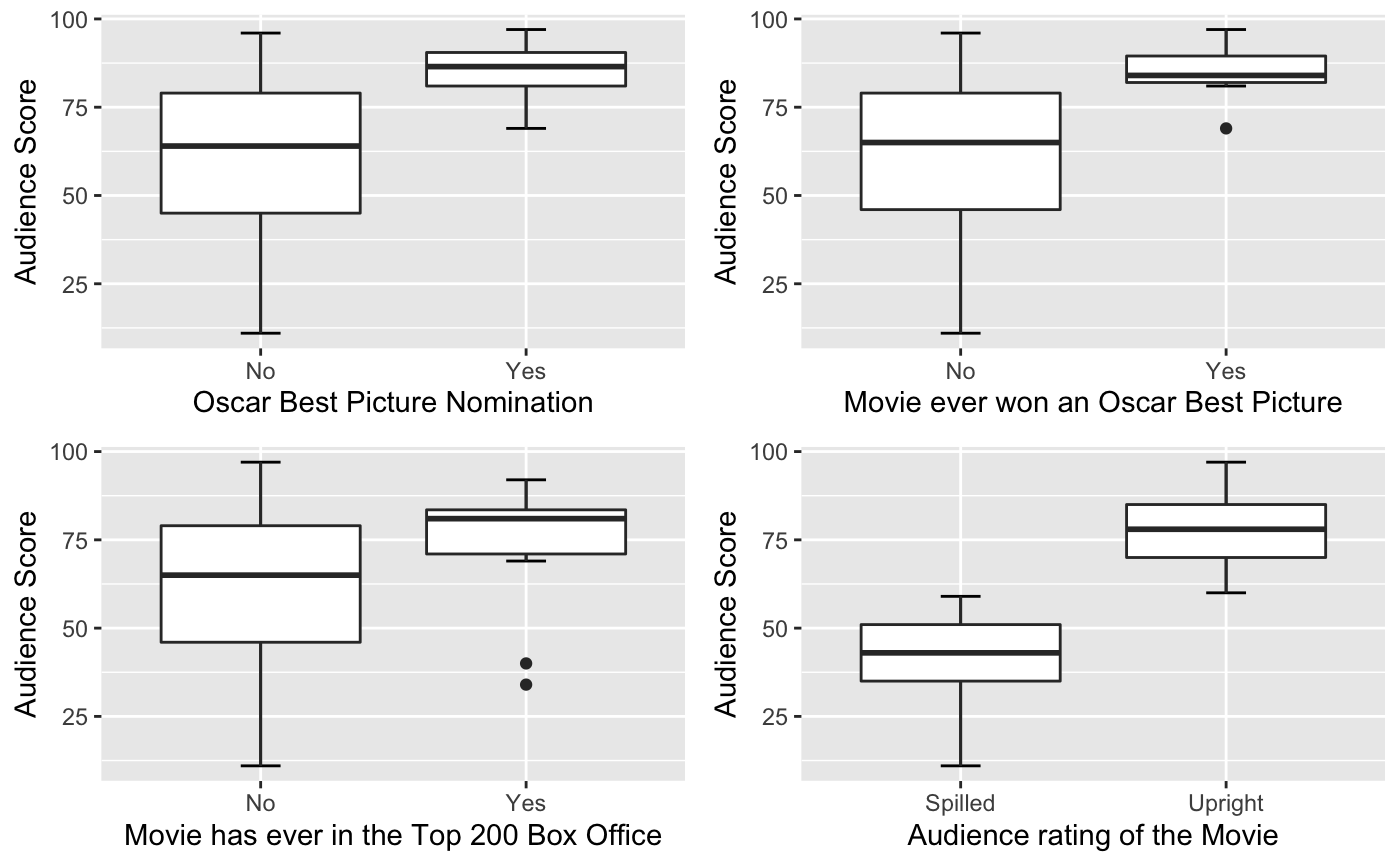
\includegraphics[scale=0.32]{boxplot2.png}
\label{fig: 8}
\end{center}
\end{figure}

The boxplot (Figure~\ref{fig: 8} lower right) depicting the distribution of audience score by the audience rating that the movie received on Rotten Tomatoes. Based on this plot, it seems movies that received an "Upright" audience rating on Rotten Tomatoes tend to receive higher audience scores in comparison to movies that received a "Spilled" audience rating. Moreover, the box of movies that received an "Upright" audience rating on Rotten Tomatoes is completely above the box of movies that received a "Spilled" audience rating. This indicates that there is a significant difference between those two groups and it is highly possible that audience rating could be a good predictor variable of the audience score.

Figure~\ref{fig: 9} includes another four boxplots of the distribution of audience score as grouped by another four categorical predictor variables. To sum up, there seems to be no significant difference between the distributions of audience score grouped by whether or not the actors of movies ever won an Oscar, as well as whether or not the actresses of the movies ever won an Oscar. This may indicates that those two categorical variables may not be a good predictor variable for the audience score (Two Sample T-Test show P-value greater than 0.05). In addition, there seems to be little difference between the distribution of audience score grouped by whether or not movie director has ever won an Oscar, but the difference is very small (although it passed the Two Sample T-Test with a P-value = 0.01617). This difference indicates that movies that have a director who won an Oscar at least once during his or here career seem to receive higher audience score in comparison to movies that have a director who has never won an Oscar. I am going to keep those variables and the model selection process will decide which variables will be selected into the model anyway.

\begin{figure}[htbp]
\begin{center}
\caption{Boxplots of Audience Score vs. Best Actor Win, Audience Score vs. Best Actress Win, Audience Score vs. Best Director Win, Audience Score vs. Type of the Movie}
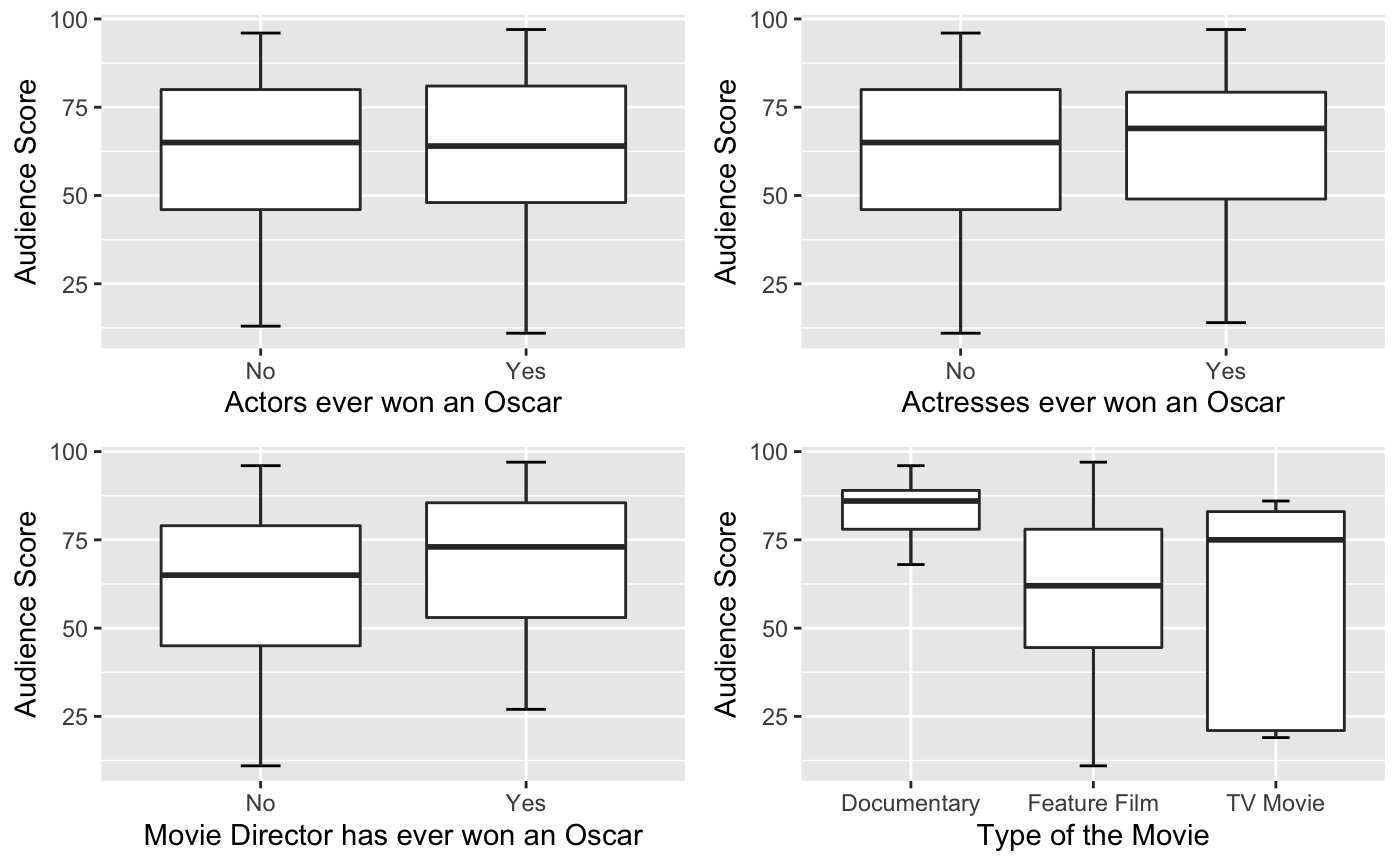
\includegraphics[scale=0.32]{boxplot3.png}
\label{fig: 9}
\end{center}
\end{figure}

The boxplot (Figure~\ref{fig: 9} lower right) depicting the distribution of the audience score by movie type (Documentary, Feature Film, and TV Movie) indicates that Documentary tend to receive higher audience scores in comparison to Feature Film and TV Movies. Moreover, the distribution of audience score by Feature Film is fairly symmetric, but the distribution of audience score for both Documentary and TV Movie is skewed to the left, which indicates that the majority of audience scores for Documentary and TV Movie are lying below the median level. 

\begin{figure}[htbp]
\begin{center}
\caption{Boxplot of Audience Score vs. Critics Rating of the Movie}
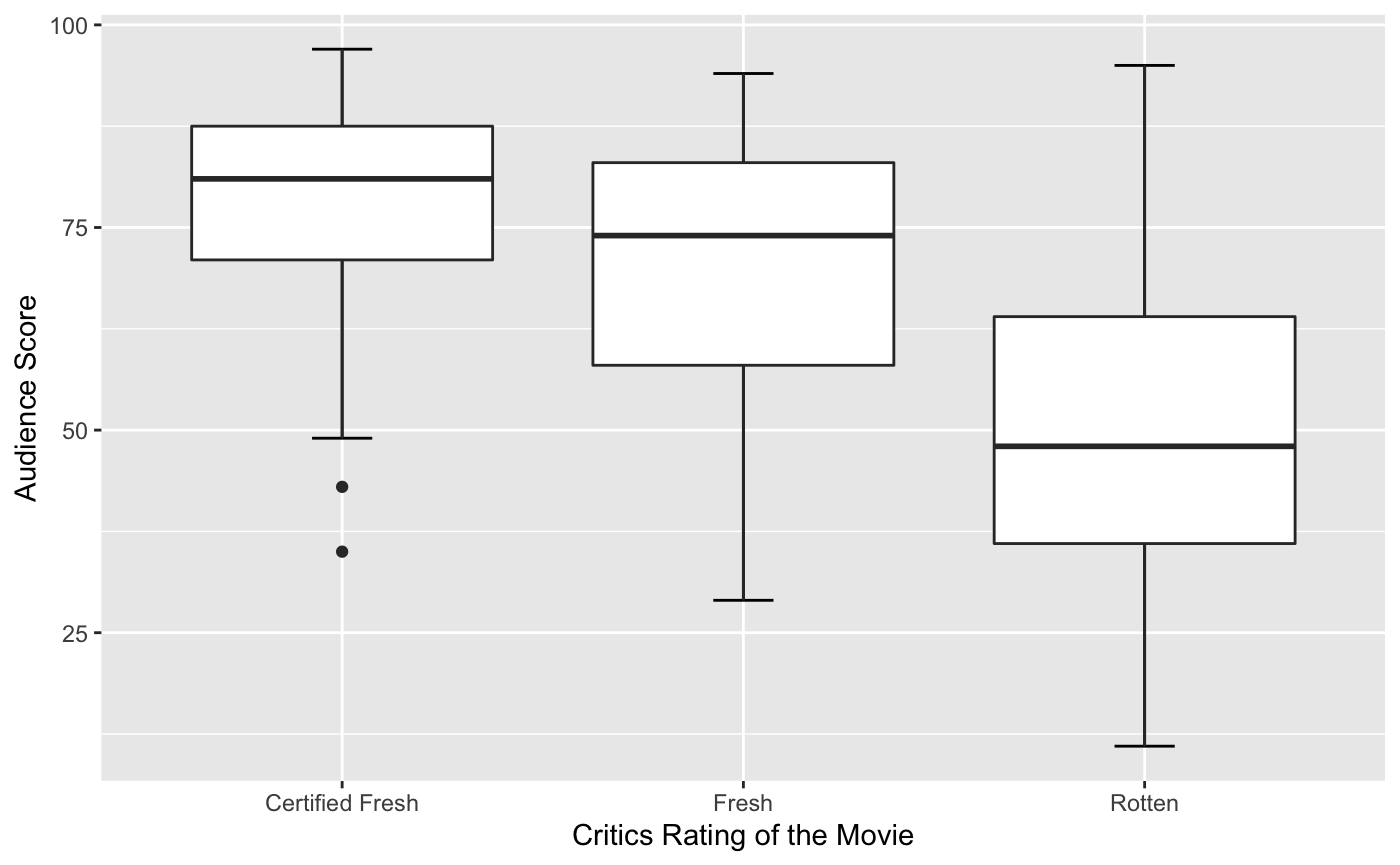
\includegraphics[scale=0.32]{boxplot4.png}
\label{fig: 10}
\end{center}
\end{figure}

The last boxplot (Figure~\ref{fig: 10}) depicting the distribution of the audience score by three levels of critics rating on Rotten Tomatoes, which are "Certified Fresh", "Fresh" and "Rotten". The plot tends to show that movies that receive a "Certified Fresh" seem to receive higher audience score compared to movies that received a "Fresh" or "Rotten". The distribution of audience score for movies received either "Certified Fresh" or "Fresh" are skewed to the left, indicating that the majority of audience scores are lying below the median level, while movies received "Rotten" seems to be skewed to the right. The difference between movies with either a "Certified Fresh" or a "Fresh" on critics rating and movies with a "Rotten" critics rating in terms of mean audience score is quite significant (as shown in Two-Sample T-Test). To be specific, the audience score fall into the bottom 25\% of movies with "Certified Fresh" critics rating is somewhat higher than the mean and median audience score of movies with "Rotten" critics rating. Therefore, the critics rating on Rotten Tomatoes may also be a good predictor for movie's audience score.

In the next section, I am going to perform the model selection to decide what variables should be kept in the model.



\newpage
\section{Modeling}
\subsection{Multicollinearity between Numerical Variables}
After exploring the data, the next step is to check if there exists any col-linearity within the numerical explanatory variables. I created a correlation matrix to understand the correlation between those variables. In the Table~\ref{tab: 1}, it seems that the critics scores and IMDB rating are highly correlated, with a correlation coefficient equals to 0.765. The high correlation between those two variables mean that if both two variables are added to the model, it will add redundant information and complicate model estimation. Therefore, one of the variables have to be remove from the analysis. To decide which of those two predictors will be removed from our analysis, I run two separate regression. The $R^2$ for the estimated regression model between audience score and IMDB rating is 0.7481, which is higher compared to the $R^2$ (0.4951) for the regression model between audience score and critics score. Therefore, I decide to keep IMDB rating in the analysis and remove the critics scores.
% Table created by stargazer v.5.2.2 by Marek Hlavac, Harvard University. E-mail: hlavac at fas.harvard.edu
% Date and time: Wed, Nov 18, 2020 - 22:58:39
\begin{table}[!htbp] \centering 
  \caption{Correlation Table for Numerical Variables} 
  \label{tab: 1} 
\begin{tabular}{@{\extracolsep{5pt}} ccccc} 
\\[-1.8ex]\hline 
\hline \\[-1.8ex] 
 & runtime & imdb\_rating & imdb\_num\_votes & critics\_score \\ 
\hline \\[-1.8ex] 
runtime & $1$ & $0.268$ & $0.347$ & $0.172$ \\ 
imdb\_rating & $0.268$ & $1$ & $0.332$ & $0.765$ \\ 
imdb\_num\_votes & $0.347$ & $0.332$ & $1$ & $0.210$ \\ 
critics\_score & $0.172$ & $0.765$ & $0.210$ & $1$ \\ 
\hline \\[-1.8ex] 
\end{tabular} 
\end{table} 

\subsection{Model Selection}
I used the Forward Stepwise Selection with both AIC and BIC method to decide if some predictors should be removed. The AIC identified 6 covariates, which are IMDB rating, audience rating on Rotten Tomatoes, genre, movie's run time, movie ever received an Oscar Best Picture nomination and movie's actress ever won an Oscar award. The BIC identified only 2 covariates, which are IMDB rating and audience rating on Rotten Tomatoes. It is not surprising because BIC imposes additional penalty for more complexity in the model and it tends to produce a more easily interpretable model. To pay a close look on those two models, the Adjusted $R^2$ for the BIC suggested model is 0.8821, while the Adjusted $R^2$ for the AIC suggested model is 0.8861. Although the latter model has a higher $R^2$ (which is consistent with our theory since AIC is better for prediction), I prefer choosing the BIC suggested model. This is due to the fact that AIC adds 4 more covariates into the model but only improved 0.004 in terms of Adjusted $R^2$. While using the model suggested by AIC does make better prediction, it requires us to collect more information. Let's do model diagnostics for the model suggested by BIC.
\subsection{Model Diagnostics}
\subsubsection{Outliers, Leverage Values and Influential Points}
Frequently in regression analysis applications, the data set contains some cases that are outlying or extreme; that is, the observation for these cases are well separated from the remainder of the data. These outlying cases may involve large residuals and often have dramatic effects on the fitted least squares regression function. Therefore, it is important to study the outlying cases carefully and decide whether they should be retained or eliminated. A case may be outlying or extreme with respect to its Y value, its X values or both.

I first identify the outlying Y observations as those cases whose studentized deleted residuals are large in absolute value. By doing so, we can conduct a formal test by means of the Bonferroni test procedure of whether the case with the largest absolute studentized residual is an outlier. The null for this test is that the observation is not an outlier. Based on the results, there are no outliers. While observation 126 is the most extreme observation in our data set, it isn't an outlier, as the null hypothesis cannot be rejected with a p-value = 0.22369. 

Next, I am going to identifying Outlying X observations. In particular, the diagonal elements of the hat matrix are a useful indicator in a multivariable setting of whether or not a case is outlying with respect to its X values. Using the Build-in `influence.measures` command, 18 cases were identified as outlying ones with respect to the pattern of the X values (calculating cutoff points by hand identified even more cases), as shown in Figure~\ref{fig: 11}. Nevertheless, it is necessary to point out that case with high leverage doesn't mean it is an influential point. Therefore, after identifying cases that are outlying with respect to their Y values and/or their X values, the next step is to ascertain whether or not those outlying cases are influential. 

\begin{figure}[htbp]
\begin{center}
\caption{Index Plot of Hat Values}
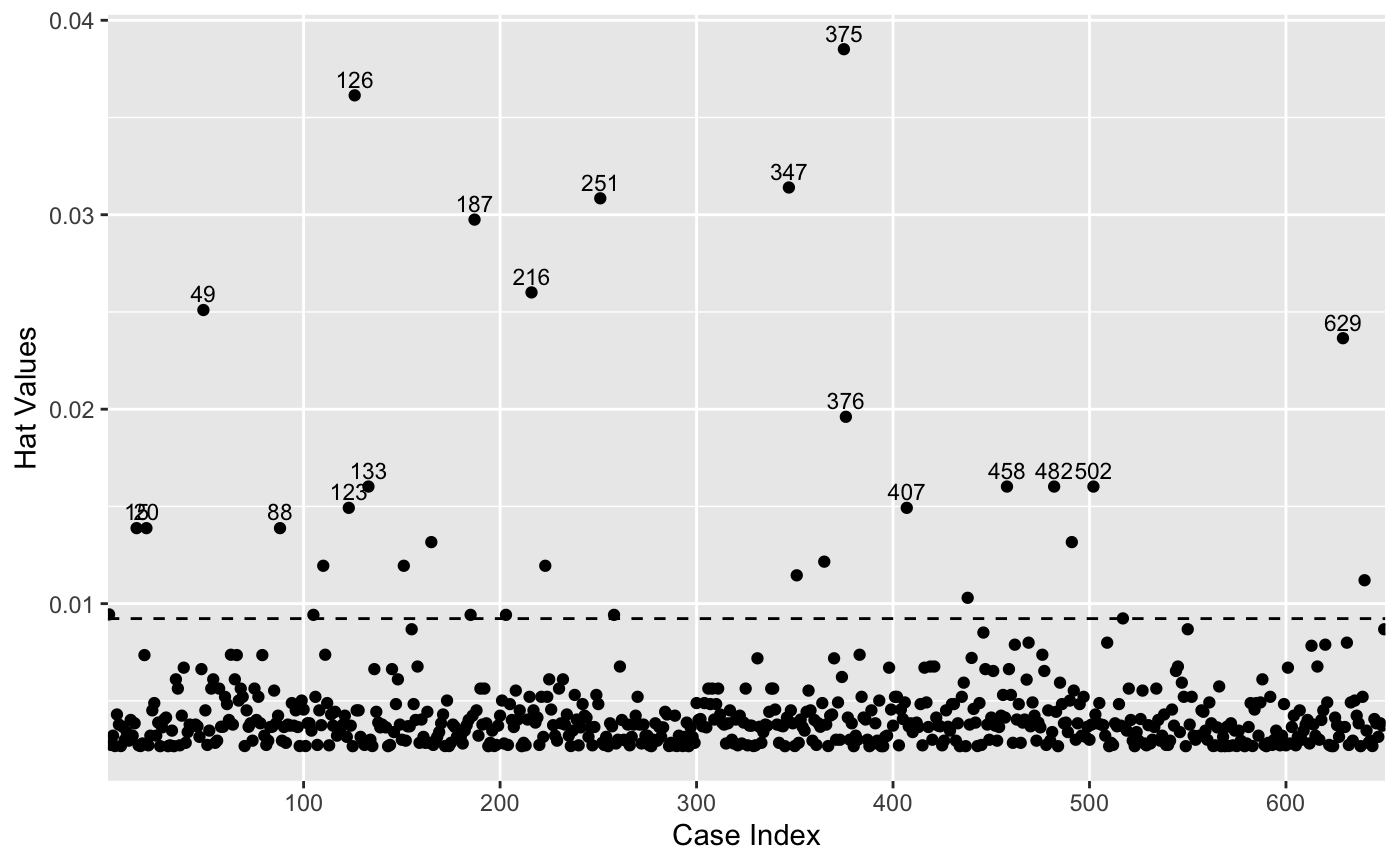
\includegraphics[scale=0.32]{leverage_points.png}
\label{fig: 11}
\end{center}
\end{figure}

We shall consider a case to be influential if its exclusion causes major changes in the fitted regression function. There are multiple ways to measure of influences, such as DFFITS, Cook's distance and DFBETAS. The basic idea behind each of these measures is the same, namely to delete the observations one at a time, each time refitting the regression model on the remaining $n-1$ observations. Then, we compare the results using all $n$ observations to the results with $i^{th}$ observation deleted to see how much influence the observation has on the analysis. Here, I am using Cook's Distance to check the influence of the $i^{th}$ case on all $n$ fitted values. There are multiple guidelines for deciding when a Cook's distance measure is large enough to warrant treating a data point as influential. Here, I am using a more theoretical guideline, as it has been found useful to relate $D_{i}$ to the $F(p, n-p)$ distribution and ascertain the corresponding percentile value. If the percentile value is near 50 percent or more, the fitted values obtained with and without the $i^{th}$ case should be considered to differ substantially, implying that the $i^{th}$ case has a major influence on the fit of the regression function.

In our case, there are no observation that has Cook's Distance larger than the cutoff point. Therefore, considering no outlying Y observations and influential points, I will keep all observations in the data set and move to check OLS assumptions, or Gauss Markov Assumptions. If all assumptions are met, then the Ordinary Least Squares estimate for regression coefficients give us the Best Linear Unbiased Estimators (\textbf{BLUE}). 

\subsubsection{Check OLS Assumptions}
\textbf{Assumption 1}: The regression model is linear in the coefficients and the error term.

To check the first assumption, we could plot the residuals versus individual independent variables (usually numeric) to see if any systematic patterns have been revealed. In this case, I am going to show the plot of residuals versus the IMDB rating. Based on Figure~\ref{fig:12}, i didn't see any systematic pattern. Therefore, the first assumption is met.

\begin{figure}[htbp]
\begin{center}
\caption{Plot of Residuals against IMDB Rating}
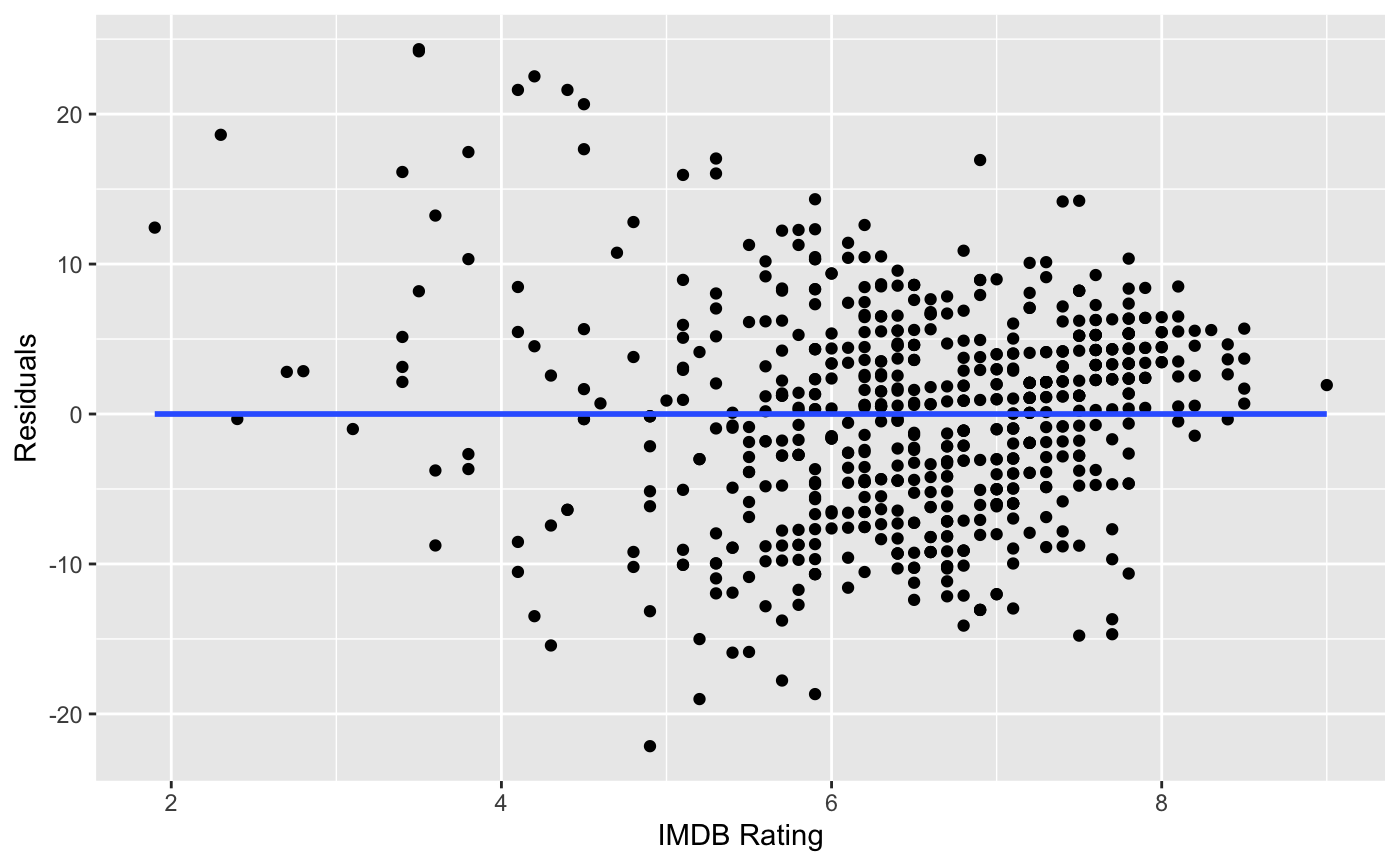
\includegraphics[scale=0.3]{linearity.png}
\label{fig:12}
\end{center}
\end{figure}

\textbf{Assumption 2}:  The error term are normally distributed with a mean of zero.

The error term accounts for the variation in the response variable that the predictor variables do not explain. To check this assumption, we could either plot a histogram of residuals or a Normal Q-Q plot. I used both two plots and presented in Figure~\ref{fig:13}. It looks like the residuals is distributed with a mean of zero, but due to the fact that the median is somewhat greater than the mean. It is a little bit left-skewd. The Normal Q-Q plot also shows roughly normal, that the majority of the points lie on the 45 degree line, but the ends start to deviate.

Formal tests, such as Shapiro-Wilk and Anderson-Darling Normality test could be used to test the normality of the residuals. Due to the low p-value for both Anderson-Darling Normality Test and Shaprio-Wilk Test, residuals do not follow a normal distribution. Nevertheless, It is possible that with large sample-sized data set, the normality test may detect trivial departures from the null hypothesis, which resulting in the rejection of the null hypothesis. I decided not to fix this normally distributed issues as the sample size is quite large here ($n=650$). Indeed, the Gauss Markov Theorem does not require the error term follows a normal distribution.

\begin{figure}[htbp]
\begin{center}
\caption{Distribution of Residuals}
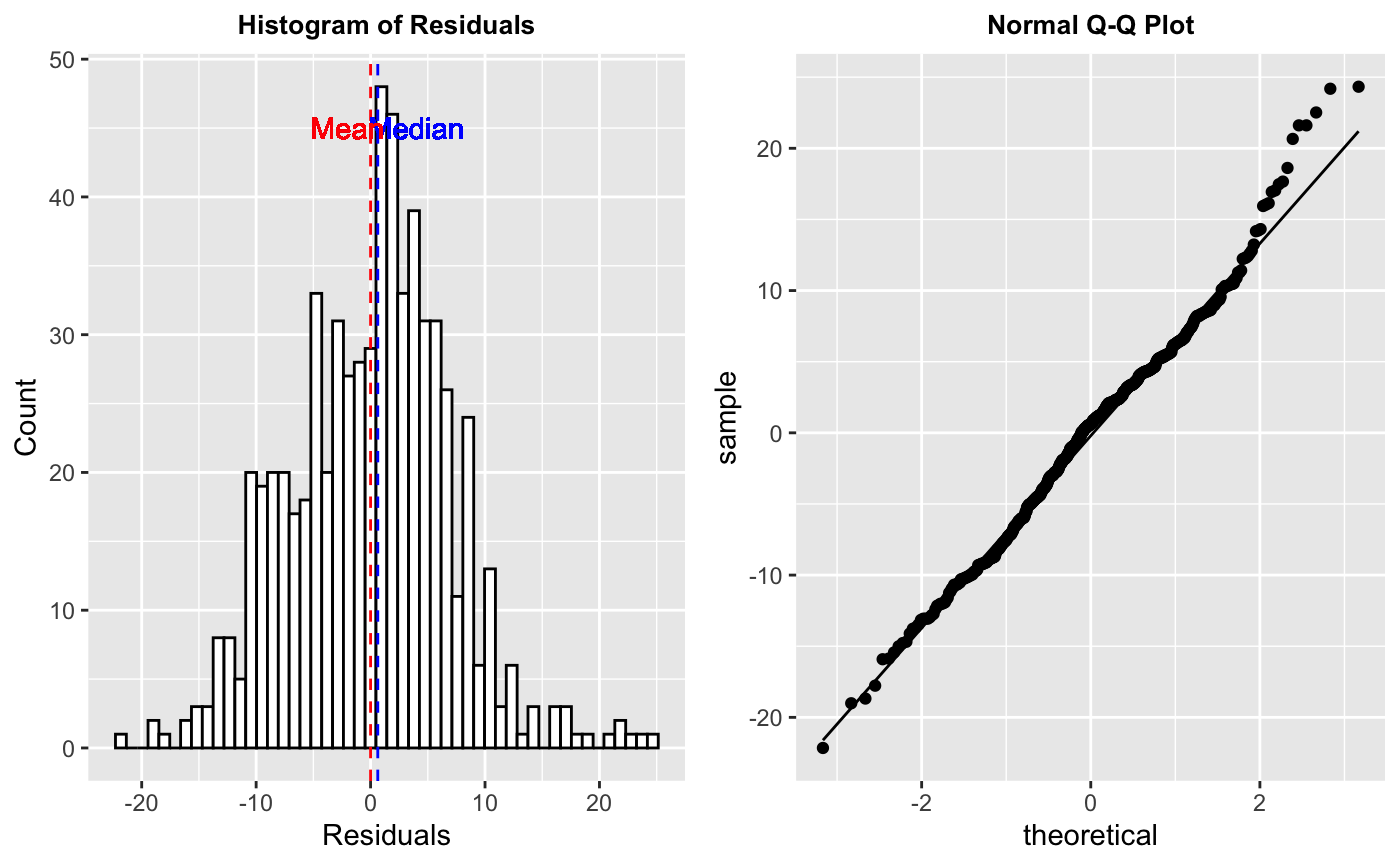
\includegraphics[scale=0.32]{residuals_check.png}
\label{fig:13}
\end{center}
\end{figure}

\textbf{Assumption 3}: The error term has a constant variance, known as homoscedasticity.

OLS requires the variance of the errors should be consistent for all observations. That is, their variance does not change across different levels of the predictors. If the residuals do not satisfy the constant variance assumption, then we face an issue of heteroskedasticity, leading the standard errors and confidence intervals be adversely affected (Heteroskedasticity reduces the precision or efficiency of the estimates of the OLS estimators), irrespective of whether the sample size is large or not. To check this assumption, the easiest way is to create a residuals versus fitted value plot. If there is no systematic pattern for the residuals against the fitted values, we conclude homoscedasticity. Otherwise, we conlude heteroskedasticity. 

The Figure~\ref{fig: 14} exhibits a megaphone shape. There is more variation in the lower level of fitted audience scores. Therefore, I confirmed heteroskedasticity and the assumption of constant variance for the error terms is violated. Moreover, we can also use Breusch-Pagan Test to check the  heteroskedasticity. The null hypothesis is that the error term has a constant variance (homoscedasticity). Due to the low p-value, we should reject the null hypothesis and conclude the heteroskedasticity.

\begin{figure}[htbp]
\begin{center}
\caption{Plot of OLS Standardized Residuals versus Fitted Values}
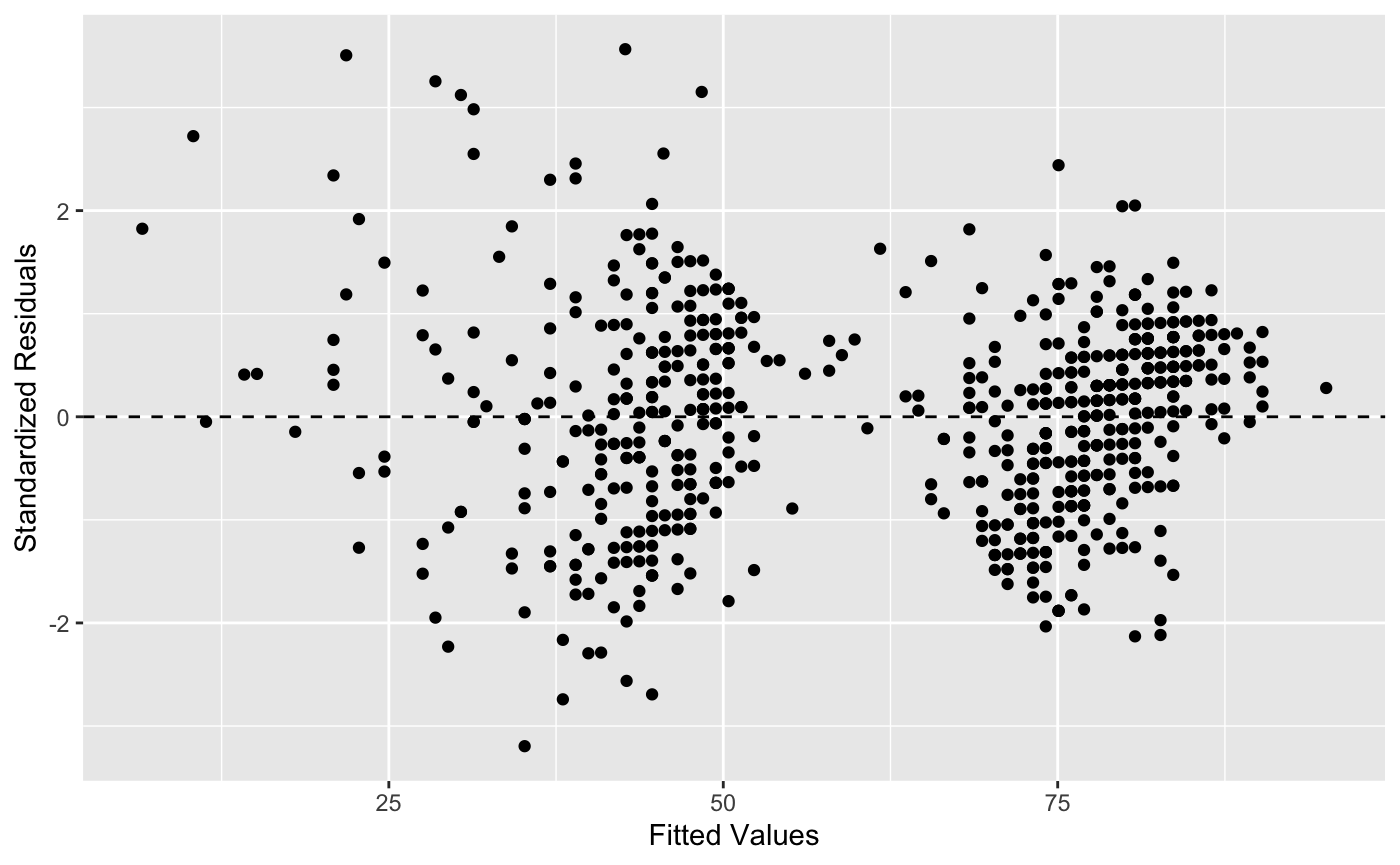
\includegraphics[scale=0.3]{ols_residuals.png}
\label{fig: 14}
\end{center}
\end{figure}

\textbf{Assumption 4}: The error terms are mutually independent (No autocorrelation).

If this assumption is violated, we usually face a serial correlation or autocorrelation problem. This usually appears in a time-series analysis. We could graph the residuals in the order that the data were collected to assess this assumption. If a "sine" type of curve is observed, then it is highly likely we do have an autocorrelation problem. To check this assumption, I use the Durbin-Watson test, and the null hypothesis of this test is that there is no autocorrelation. In our case, the p-value of this test is 0.2705, which is greater than 0.05. Therefore, I conclude there is no autocorrelation issue.

To sum up, our OLS model does face a hetroskedasticity problem, which reduces the efficiency of the OLS estimators. Therefore, it is necessary to fix this problem.

\subsection{Feasible Generalized Least Squares (FGLS)}
In practice, if the form of heteroskedasticity is known, a Weighted Least Squares (WLS) appraoch can be used to remedy this issue. Nevertheless, in reality, we usually don't know the variance of error terms, therefore, it is more practical to use the Feasible Generalized Least Squares (FGLS) approach. 	When the weighting function is modeled an estimated from data, the resulting estimated weights ($\widehat{h_{i}}$) are the bases for FGLS. After using the FGLS apprach (I am only doing the FGLS once, you can also iterate until regression coefficients are stable), I re-plotted the standardized residuals versus fitted values. 

Using Feasible GLS, according to the the Figure~\ref{fig: 15}, it looks much better (Although 
heteroskedasticity may still exists, it is much better improved) and it has a higher Adjusted R-Squared (0.889). 

\begin{figure}[htbp]
\begin{center}
\caption{Plot of FGLS Standardized Residuals versus Fitted Values}
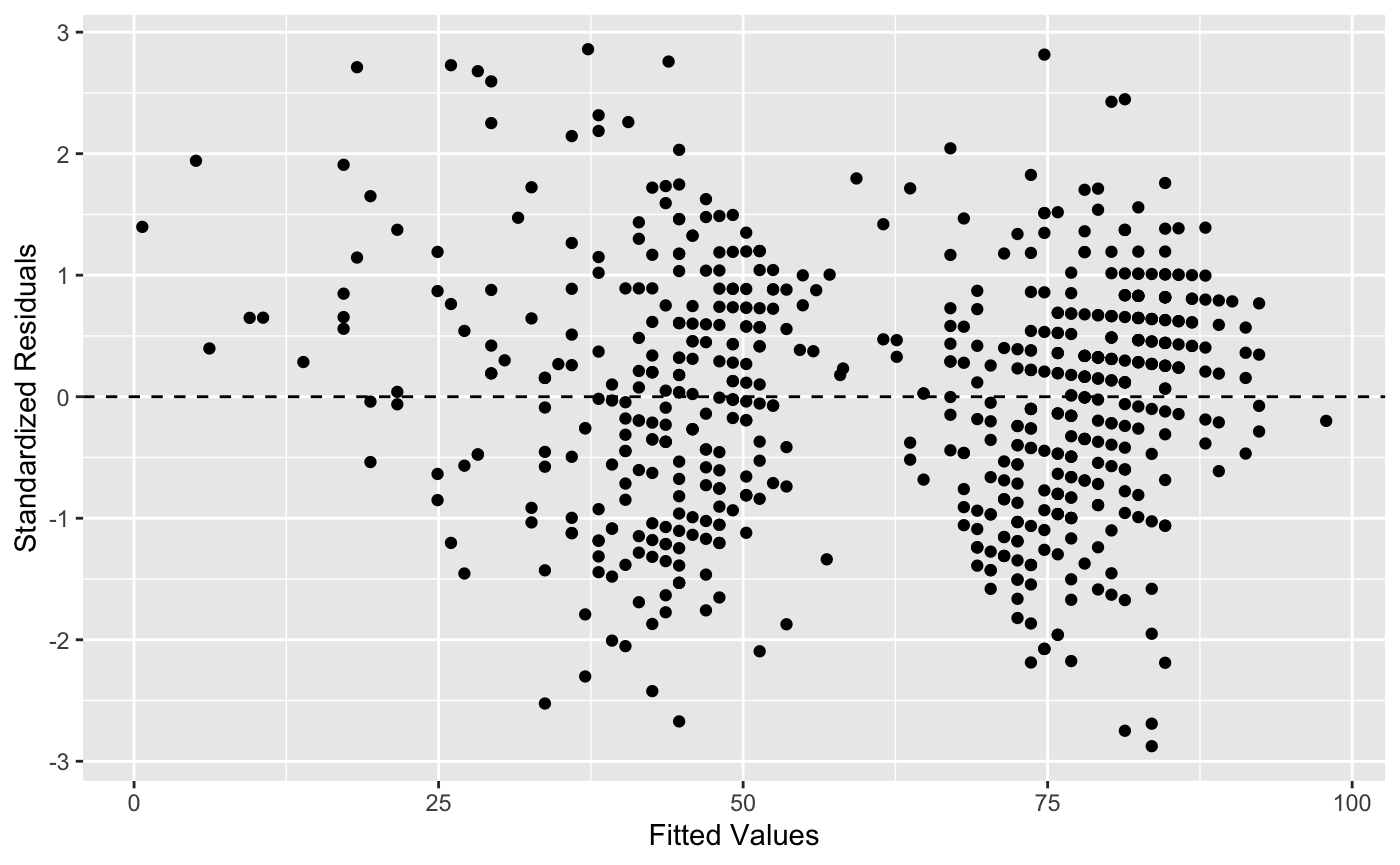
\includegraphics[scale=0.3]{fgls_residuals.png}
\end{center}
\label{fig: 15}
\end{figure}
\mbox{~} %need at least null to create a page
\newpage

\section{Regression Results and Prediction}
\subsection{Interpretation}
The final regression results are presented in Table~\ref{tab: 2}. Here, I am just going to interpret the OLS results:
\vspace{-0.5cm}
\begin{itemize}
\setlength\itemsep{-0.5em}
\item Intercept (-11.532) is the estimated audience score on Rotten Tomatoes for a movie with zero IMDB rating and audience rating categorized as Spilled. It does not provide any meaningful interpretation here.
\item IMDB Rating coefficient (9.527): Holding all other variables constant, for every one unit increase in IMDB rating, the model predicts the audience score is expected to increase  9.527 on average.
\item Audience Rating Upright coefficient (20.858): Holding all other variables constant, the model predicts that a movie with a rating with "Upright" is 20.858 higher in audience score on average than a movie rating as "Spilled".
\item $R^2$ (0.882): 88.2\% of the variability in audience score can be explained by the model.
\end{itemize}

Compared to the regression results using OLS, the FGLS estimators do not change significantly (coefficients for the predictor variables do not change their signs) and both two predictors are still strongly significant at 0.01 level. The coefficient of the IMDB rating increased from 9.527 to 11.018 while the coefficient of audience rating decreased from 20.856 to 18.966. The $R^2$ increased a little bit from 0.882 to 0.889.
\begin{table}[!htbp] \centering 
  \caption{Regression Results} 
  \label{tab: 2} 
\begin{tabular}{@{\extracolsep{5pt}}lcc} 
\\[-1.8ex]\hline 
\hline \\[-1.8ex] 
 & \multicolumn{2}{c}{\textit{Dependent variable:}} \\ 
\cline{2-3} 
\\[-1.8ex] & \multicolumn{2}{c}{Audience Score} \\ 
 & OLS & FGLS \\ 
\\[-1.8ex] & (1) & (2)\\ 
\hline \\[-1.8ex] 
 IMDB Rating & 9.527$^{***}$ & 11.018$^{***}$ \\ 
  & (0.350) & (0.376) \\ 
  & & \\ 
 Audience Rating-Upright & 20.858$^{***}$ & 18.966$^{***}$ \\ 
  & (0.767) & (0.761) \\ 
  & & \\ 
 Constant & $-$11.532$^{***}$ & $-$20.258$^{***}$ \\ 
  & (2.006) & (2.231) \\ 
  & & \\ 
\hline \\[-1.8ex] 
Observations & 650 & 650 \\ 
R$^{2}$ & 0.882 & 0.889 \\ 
Adjusted R$^{2}$ & 0.882 & 0.889 \\ 
Residual Std. Error (df = 647) & 6.949 & 1.738 \\ 
F Statistic (df = 2; 647) & 2,427.986$^{***}$ & 2,599.298$^{***}$ \\ 
\hline 
\hline \\[-1.8ex] 
\textit{Note:}  & \multicolumn{2}{r}{$^{*}$p$<$0.1; $^{**}$p$<$0.05; $^{***}$p$<$0.01} \\ 
\end{tabular} 
\end{table}

\subsection{Prediction}
I am going to predict the audience score for a new movie that has not been used to fit the model. The movie I choose is "The Incredible Hulk", which was produced by Universal Pictures in 2008. I extracted the audience rating from Rotten Tomatoes and IMDB rating from IMDB (6.7, which lies inside the range of the values of the predictor variables in our model). The true audience 
score for this movie is 70.
\vspace{-0.5cm}
\subsubsection{OLS estimates:}
The OLS model predicts movie "The Incredible Hulk" will have an audience score at approximately 73.16. The model predicts, with 95\% confidence, that the movie is expected to have an audience score between 59.49 and 86.83. The prediction interval contains the actual audience score for this movie.
\vspace{-0.5cm}
\subsubsection{FGLS estimates:}
The FGLS model predicts movie "The incredible Hulk" will have an audience score at approximately 
72.53. The model predicts, with 95\% confidence, that the movie is expected to have an audience score between 60.06 and 85.00. The fitted value is much closer to the actual audience value compared to the OLS estimation and the prediction interval contains the actual audience score as well. The FGLS confidence interval is narrower than OLS. This is another way to show that FGLS is more efficient than OLS, althuough its estimates may not be \textbf{BLUE}.
\newpage

\section{Conclusion}
In conclusion, the model developed in this project demonstrates that it is possible to predict a move's popularity, as measured by audience's score on Rotten Tomatoes, with only two predictor variables, which are IMDB rating and Audience Rating (Categorical Variable: Spilled, Upright) on Rotten Tomatoes. The findings could be quite informative to movie producers so that they could use similar methods to predict their movies' popularity. This project also demonstrates that conducting a exploratory data analysis was of great help in getting general idea of the data set, as well as the relationship between the response variable and the predictor variable. Although the process of the EDA is quite time-consuming, all the efforts will be rewarded. 

One of the major tasks of this project is dealing with the heteroskedasticity problem of the OLS model. By taking the Feasible Generalized Least Squares (FGLS) approach, we do achieve some improvements, as shown on the standardized residuals versus fitted values plot after running FGLS. Therefore, It is always better to try to fix the issue over ignoring heteroskedasticity and estimating directly by OLS. 

What's more, I conducted outliers, leverage values and influential points test in the model diagnostics section and finally decided not to remove any observations from the original data set. Admittedly, if you use different guidelines on those tests, it will give you very different results. For instance, in terms of Cook's Distance, I took a more theoretical way (F-Distribution as cutoff) to identify the influential points and do not find any observations have $D_{i}$ larger than the cutoff point. If you take alternative cutoff point, like $\frac{4}{n}$, you will find more influential points. Making decisions to remove outliers and influential points is hard, and it is indeed not a statistical problem at most of time. You must give sufficient reasons explain why you want to remove those observation, like data entry issue. If you cannot legitimately remove outliers, using Robust Regression or Bootstrapping techniques may be more appropriate. Those methods have not been explored in this project.

Finally, the potential shortcoming is that the sample data we have is not representative. This could be a very critical issue. As shown in the EDA section Figure~\ref{fig: 3}, nearly 46.92\% of movies in the data are drama movies. Therefore, the results may be biased toward drama movies. On this occasion, it is necessary to collect more observations so that we could capture more variability in the population data and improves model's accuracy. 
\newpage
\bibliographystyle{apa}
\bibliography{literature}

\end{document}